\subsection{Generic lists} \label{qlist}
The provided list implementation uses a generic \textit{doubly-linked} approach in which each node, apart from storing its data, has two link pointers. The first link points to the previous node in the list and the second link, points to the next node in the list. The first node of the list has its previous link pointing to \lstinline{NULL}, similarly, the last node of the list has its next node pointing to \lstinline{NULL}. \\
The list data-structure, referenced through an object of type \lstinline{qList_t} \index{\lstinline{qList_t}} also has a \textit{head} and a \textit{tail} pointer, to allow fast operations on boundary nodes.

\begin{figure}[H]
    \centering
    \tikzset{every picture/.style={line width=0.75pt}} %set default line width to 0.75pt        
    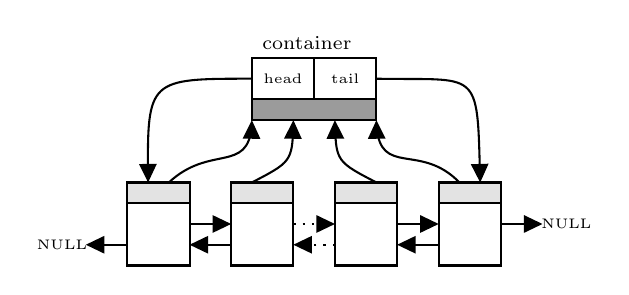
\begin{tikzpicture}[x=0.75pt,y=0.75pt,yscale=-1,xscale=1]
        \draw   (200,110) -- (230,110) -- (230,150) -- (200,150) -- cycle ;
        \draw    (230,130) -- (247,130) ;
        \draw [shift={(250,130)}, rotate = 180] [fill={rgb, 255:red, 0; green, 0; blue, 0 }  ][line width=0.08]  [draw opacity=0] (8.93,-4.29) -- (0,0) -- (8.93,4.29) -- cycle    ;
        \draw    (200,140) -- (183,140) ;
        \draw [shift={(180,140)}, rotate = 360] [fill={rgb, 255:red, 0; green, 0; blue, 0 }  ][line width=0.08]  [draw opacity=0] (8.93,-4.29) -- (0,0) -- (8.93,4.29) -- cycle    ;
        \draw   (250,110) -- (280,110) -- (280,150) -- (250,150) -- cycle ;
        \draw  [dash pattern={on 0.84pt off 2.51pt}]  (280,130) -- (297,130) ;
        \draw [shift={(300,130)}, rotate = 180] [fill={rgb, 255:red, 0; green, 0; blue, 0 }  ][line width=0.08]  [draw opacity=0] (8.93,-4.29) -- (0,0) -- (8.93,4.29) -- cycle    ;
        \draw    (250,140) -- (233,140) ;
        \draw [shift={(230,140)}, rotate = 360] [fill={rgb, 255:red, 0; green, 0; blue, 0 }  ][line width=0.08]  [draw opacity=0] (8.93,-4.29) -- (0,0) -- (8.93,4.29) -- cycle    ;
        \draw   (300,110) -- (330,110) -- (330,150) -- (300,150) -- cycle ;
        \draw    (330,130) -- (347,130) ;
        \draw [shift={(350,130)}, rotate = 180] [fill={rgb, 255:red, 0; green, 0; blue, 0 }  ][line width=0.08]  [draw opacity=0] (8.93,-4.29) -- (0,0) -- (8.93,4.29) -- cycle    ;
        \draw  [dash pattern={on 0.84pt off 2.51pt}]  (300,140) -- (283,140) ;
        \draw [shift={(280,140)}, rotate = 360] [fill={rgb, 255:red, 0; green, 0; blue, 0 }  ][line width=0.08]  [draw opacity=0] (8.93,-4.29) -- (0,0) -- (8.93,4.29) -- cycle    ;
        \draw   (350,110) -- (380,110) -- (380,150) -- (350,150) -- cycle ;
        \draw    (380,130) -- (397,130) ;
        \draw [shift={(400,130)}, rotate = 180] [fill={rgb, 255:red, 0; green, 0; blue, 0 }  ][line width=0.08]  [draw opacity=0] (8.93,-4.29) -- (0,0) -- (8.93,4.29) -- cycle    ;
        \draw    (350,140) -- (333,140) ;
        \draw [shift={(330,140)}, rotate = 360] [fill={rgb, 255:red, 0; green, 0; blue, 0 }  ][line width=0.08]  [draw opacity=0] (8.93,-4.29) -- (0,0) -- (8.93,4.29) -- cycle    ;
        \draw   (260,50) -- (290,50) -- (290,70) -- (260,70) -- cycle ;
        \draw    (320,60) .. controls (369.74,60.99) and (368.55,54.07) .. (369.93,107.52) ;
        \draw [shift={(370,110)}, rotate = 268.47] [fill={rgb, 255:red, 0; green, 0; blue, 0 }  ][line width=0.08]  [draw opacity=0] (8.93,-4.29) -- (0,0) -- (8.93,4.29) -- cycle    ;
        \draw    (260,60) .. controls (210.51,60) and (209.52,60) .. (209.97,107.06) ;
        \draw [shift={(210,110)}, rotate = 269.43] [fill={rgb, 255:red, 0; green, 0; blue, 0 }  ][line width=0.08]  [draw opacity=0] (8.93,-4.29) -- (0,0) -- (8.93,4.29) -- cycle    ;
        \draw   (290,50) -- (320,50) -- (320,70) -- (290,70) -- cycle ;
        \draw  [fill={rgb, 255:red, 155; green, 155; blue, 155 }  ,fill opacity=1 ] (260,70) -- (320,70) -- (320,80) -- (260,80) -- cycle ;
        \draw    (220,110) .. controls (239.78,91.53) and (258.17,105.78) .. (259.88,82.67) ;
        \draw [shift={(260,80)}, rotate = 451.07] [fill={rgb, 255:red, 0; green, 0; blue, 0 }  ][line width=0.08]  [draw opacity=0] (8.93,-4.29) -- (0,0) -- (8.93,4.29) -- cycle    ;
        \draw    (260,110) .. controls (278.52,100.36) and (279.45,99.88) .. (279.93,82.83) ;
        \draw [shift={(280,80)}, rotate = 451.44] [fill={rgb, 255:red, 0; green, 0; blue, 0 }  ][line width=0.08]  [draw opacity=0] (8.93,-4.29) -- (0,0) -- (8.93,4.29) -- cycle    ;
        \draw    (320,110) .. controls (301.47,100.36) and (300.55,99.88) .. (300.07,82.83) ;
        \draw [shift={(300,80)}, rotate = 448.56] [fill={rgb, 255:red, 0; green, 0; blue, 0 }  ][line width=0.08]  [draw opacity=0] (8.93,-4.29) -- (0,0) -- (8.93,4.29) -- cycle    ;
        \draw    (360,110) .. controls (341.18,90.56) and (321.9,107.58) .. (320.12,82.86) ;
        \draw [shift={(320,80)}, rotate = 449.01] [fill={rgb, 255:red, 0; green, 0; blue, 0 }  ][line width=0.08]  [draw opacity=0] (8.93,-4.29) -- (0,0) -- (8.93,4.29) -- cycle    ;
        \draw  [fill={rgb, 255:red, 210; green, 210; blue, 210 }  ,fill opacity=0.62 ] (200,110) -- (230,110) -- (230,120) -- (200,120) -- cycle ;
        \draw  [fill={rgb, 255:red, 210; green, 210; blue, 210 }  ,fill opacity=0.62 ] (250,110) -- (280,110) -- (280,120) -- (250,120) -- cycle ;
        \draw  [fill={rgb, 255:red, 210; green, 210; blue, 210 }  ,fill opacity=0.62 ] (300,110) -- (330,110) -- (330,120) -- (300,120) -- cycle ;
        \draw  [fill={rgb, 255:red, 210; green, 210; blue, 210 }  ,fill opacity=0.62 ] (350,110) -- (380,110) -- (380,120) -- (350,120) -- cycle ;
        \draw (275,60) node  [font=\tiny] [align=left] {\lstinline{head}};
        \draw (305,60) node  [font=\tiny] [align=left] {\lstinline{tail}};
        \draw (286.5,43) node  [font=\scriptsize] [align=left] {container};
        \draw (168.5,140) node  [font=\tiny] [align=left] {\lstinline{NULL}};
        \draw (411.5,130) node  [font=\tiny] [align=left] {\lstinline{NULL}};
    \end{tikzpicture}
    \caption{Doubly-linked list implementation}
    \label{fig:qlistsfigure}
\end{figure}

Nodes should be an user-defined data structure of any number of members, however, they must be specially defined to be compatible with the provided APIs. All the user-defined nodes must have the \lstinline{qNode_MinimalFields}\index{\lstinline{qNode_MinimalFields}} definition on top of the structure. An example is shown below:
\medskip

\begin{lstlisting}[style=CStyle]
typedef struct{
    qNode_MinimalFields; /*< required for lists*/
    int a;
    int b;
    float y;
}userdata_t;
\end{lstlisting}

With this special type definition on all custom data, the application writer can take advantage of this powerful data structure. The following APIs are provided for lists management:

\noindent\hrulefill


\begin{lstlisting}[style=CStyle]
qBool_t qList_Initialize( qList_t * const list )
\end{lstlisting}

Must be called before a list is used.  This initializes all the members of the 
list object. \index{\lstinline{qList_Initialize}}

\subsubsection*{Parameters:}
\begin{itemize}
    \item \lstinline{list} : Pointer to the list being initialised. 
\end{itemize}

\subsubsection*{Return value:}
\lstinline{qTrue} on success, otherwise returns \lstinline{qFalse}. 


\noindent\hrulefill

\begin{lstlisting}[style=CStyle]
qBool_t qList_Insert( qList_t *const list, void * const node, 
                      const qList_Position_t position ){
\end{lstlisting}

Insert an item into the list. \index{\lstinline{qList_Insert}}

\subsubsection*{Parameters:}
\begin{itemize}
    \item \lstinline{list} : Pointer to the list. 
    \item \lstinline{node} : A pointer to the node to be inserted.
    \item \lstinline{position} : The position where the node will be inserted. Could be \lstinline{qList_AtFront}, \lstinline{qList_AtBack} or any other index number where the node will be inserted after.
    
    \textit{Note}: If the index exceeds the size of the list, the node will be inserted at the back.
    
    \textit{Note}: If the list is empty, the node will be inserted as the first item.
\end{itemize}

\subsubsection*{Return value:}
\lstinline{qTrue} if the item was successfully added to the list, otherwise returns \lstinline{qFalse}. 

\noindent\hrulefill

\begin{lstlisting}[style=CStyle]
void* qList_Remove( qList_t * const list, void * const node, 
                    const qList_Position_t position )
\end{lstlisting}

Remove an item from the list. \index{\lstinline{qList_Remove}}

\subsubsection*{Parameters:}
\begin{itemize}
    \item \lstinline{list} : Pointer to the list. 
    \item \lstinline{node} : A pointer to the node to be deleted (to ignore pass \lstinline{NULL} ).
    \item \lstinline{position} : The position of the node that will be deleted. Could be \lstinline{qList_AtFront}, \lstinline{qList_AtBack} or any other index number.
    
    \textit{Note}: If the \lstinline{node} argument is supplied, the removal will be only effective if the data is member of the list. If ignored or the data is not a member of the list, this function will use the \lstinline{position} instead as index for removal.
    
    \textit{Note}: If the index exceeds the size of the list, the last node  will be removed.
\end{itemize}

\subsubsection*{Return value:}
A pointer to the removed node. \lstinline{NULL} if removal can be performed.

\noindent\hrulefill

\begin{lstlisting}[style=CStyle]
qBool_t qList_IsMember( const qList_t *const list, const void *const node )
\end{lstlisting}

Check if the node is member of the list. \index{\lstinline{qList_IsMember}}

\subsubsection*{Parameters:}
\begin{itemize}
    \item \lstinline{list} : Pointer to the list. 
    \item \lstinline{node} : A pointer to the node .
\end{itemize}

\subsubsection*{Return value:}
\lstinline{qTrue} if the node belongs to the list, \lstinline{qFalse} if it is not.

\noindent\hrulefill

\begin{lstlisting}[style=CStyle]
void* qList_GetFront( const qList_t *const list ){
\end{lstlisting}

Get a pointer to the front item of the list. \index{\lstinline{qList_GetFront}}

\subsubsection*{Parameters:}
\begin{itemize}
    \item \lstinline{list} : Pointer to the list. 
\end{itemize}

\subsubsection*{Return value:}
A pointer to the front node. \lstinline{NULL} if the list is empty.

\noindent\hrulefill

\begin{lstlisting}[style=CStyle]
void* qList_GetBack( const qList_t *const list )
\end{lstlisting}

Get a pointer to the back item of the list. \index{\lstinline{qList_GetBack}}

\subsubsection*{Parameters:}
\begin{itemize}
    \item \lstinline{list} : Pointer to the list. 
\end{itemize}

\subsubsection*{Return value:}
A pointer to the front node. \lstinline{NULL} if the list is empty.


\noindent\hrulefill

\begin{lstlisting}[style=CStyle]
qBool_t qList_IsEmpty( const qList_t * const list )
\end{lstlisting}

Check if the list is empty. \index{\lstinline{qList_IsEmpty}}

\subsubsection*{Parameters:}
\begin{itemize}
    \item \lstinline{list} : Pointer to the list. 
\end{itemize}

\subsubsection*{Return value:}
\lstinline{qTrue} if the list is empty, \lstinline{qFalse} if it is not.


\noindent\hrulefill

\begin{lstlisting}[style=CStyle]
size_t qList_Length( const qList_t * const list )
\end{lstlisting}

Get the number of items inside the list. \index{\lstinline{qList_Length}}

\subsubsection*{Parameters:}
\begin{itemize}
    \item \lstinline{list} : Pointer to the list. 
\end{itemize}

\subsubsection*{Return value:}
The number of items of the list. 

\noindent\hrulefill

\begin{lstlisting}[style=CStyle]
qBool_t qList_Move( qList_t *const destination, qList_t *const source, 
                    const qList_Position_t position )
\end{lstlisting} \index{\lstinline{qList_Move}}

Moves(or merge) the entire list pointed by \lstinline{source} to the list pointed by \lstinline{destination} at location specified by \lstinline{position}. 
After the move operation, this function leaves empty the list pointed by \lstinline{source}.

\subsubsection*{Parameters:}
\begin{itemize}
    \item \lstinline{destination} : Pointer to the list where the \lstinline{source} nodes are to be moved. 
    \item \lstinline{source} : Pointer to the source list to be moved.
    \item \lstinline{position} : The position where \lstinline{source} list will be inserted. Could be \lstinline{qList_AtFront}, \lstinline{qList_AtBack} or any other index number where the list will be inserted after.
\end{itemize}

\subsubsection*{Return value:}
\lstinline{qTrue} if the move operation is performed successfully, otherwise  returns \lstinline{qFalse}.  

\noindent\hrulefill

\begin{lstlisting}[style=CStyle]
qBool_t qList_ForEach( qList_t *const list, qList_NodeFcn_t Fcn, 
                       void *arg, qList_Direction_t dir, void *NodeOffset )
\end{lstlisting} \index{\lstinline{qList_ForEach}}

Operate on each element of the list.

\subsubsection*{Parameters:}
\begin{itemize}
    \item \lstinline{list} : Pointer to the list.
    \item \lstinline{Fcn} : The function to perform over the node. 
                            
                            Should have this prototype:
                            
                            \lstinline{ qBool_t Function( qList_ForEachHandle_t h ) }
                            
                            where the \lstinline{h} its a handle of the list iterator with the following members:
                            
                            
                            \begin{itemize}
                                \item \lstinline{node} : the k-element of the list that is currently being processed in the loop.
                                \item \lstinline{arg} : same argument of the calling function.
                                \item  \lstinline{stage} : indicates the loop progress and should be checked by the application writer to perform the specific operations over the list. This variable can take the following values:
                                \begin{itemize}
                                    \item \lstinline{QLIST_WALKINIT} : When the loop is about to start. In this case, A \lstinline{NULL} value will be passed inside the \lstinline{node} member.
                                    \item \lstinline{QLIST_WALKTHROUGH} : When the loop is traversing the list.
                                    \item \lstinline{QLIST_WALKEND} :  When the loop has finished. In this case, A \lstinline{NULL} value will be passed in the \lstinline{node} member. 
                                \end{itemize}
                            \end{itemize}
                            
                            By default, \lstinline{Function} should return \lstinline{qFalse}. If a \lstinline{qTrue} value is returned, the walk through loop will be terminated.
    \item \lstinline{arg} : Argument passed to \lstinline{Fcn} through the iterator handle.
    \item \lstinline{dir} : Use one of the following options:
                            \begin{itemize}
                                \item \lstinline{QLIST_FORWARD} : to walk through the list forwards.
                                \item \lstinline{QLIST_BACKWARD} to walk through the list backwards.
                            \end{itemize}
    \item \lstinline{NodeOffset} : If available, the list walk through will start from this node.  
                   To ignore, pass \lstinline{NULL}.
\end{itemize}

\subsubsection*{Return value:}
\lstinline{qTrue} if the walk through was early terminated, otherwise returns \lstinline{qFalse}.

\noindent\hrulefill

\begin{lstlisting}[style=CStyle]
qBool_t qList_Sort( qList_t * const list, 
                    qBool_t (*CompareFcn)( qList_CompareHandle_t h ) ) 
\end{lstlisting} \index{\lstinline{qList_Sort}}

Sort the double linked list using the \lstinline{CompareFcn} function to 
determine the order.
The sorting algorithm used by this function compares pairs of adjacent nodes by calling the specified \lstinline{CompareFcn} function. The sort is performed only modifying node's links without data swapping, improving performance if nodes have a large storage.

\textit{Note:} The function modifies the content of the list by reordering its 
elements as defined by \lstinline{CompareFcn}.

\subsubsection*{Parameters:}
\begin{itemize}
    \item \lstinline{list} : Pointer to the list. 
    \item \lstinline{CompareFcn} : Pointer to a function that compares two nodes.
                    This function is called repeatedly by \lstinline{qList_Sort} to compare two nodes. It shall follow the following prototype:
                    \lstinline{qBool_t (*CompareFcn)( qList_CompareHandle_t h )}
                    
                    Taking \lstinline{h} as the conpare-handle argument with two members inside, \lstinline{n1} and \lstinline{n2}, pointing to the nodes being compared (both converted to (\lstinline{const void*}). The function defines the order of the elements by returning a Boolean data, where a \lstinline{qTrue} value indicates that element pointed by \lstinline{n1} goes after the element pointed to by \lstinline{n2}
\end{itemize}

\subsubsection*{Return value:}
\lstinline{qTrue} if at least one reordering is performed over the list. 


\noindent\hrulefill

\begin{lstlisting}[style=CStyle]
qBool_t qList_IteratorSet( qList_Iterator_t *iterator, qList_t *const list, 
                           void *NodeOffset, qList_Direction_t dir )
\end{lstlisting} \index{\lstinline{qList_IteratorSet}}

Setup an instance of the given iterator to traverse the list.

\subsubsection*{Parameters:}
\begin{itemize}
    \item \lstinline{iterator} : Pointer to the iterator instance. 
    \item \lstinline{list} : Pointer to the list.
    \item \lstinline{NodeOffset} : The start offset-node. To ignore, pass \lstinline{NULL}.
    \item \lstinline{dir} : Use one of the following options:
        \begin{itemize}
            \item \lstinline{QLIST_FORWARD} : to go in forward direction.
            \item \lstinline{QLIST_BACKWARD} : to go in backward direction.
        \end{itemize}
\end{itemize}

\subsubsection*{Return value:}
\lstinline{qTrue} on success. Otherwise returns \lstinline{qFalse}. 

\noindent\hrulefill

\begin{lstlisting}[style=CStyle]
void* qList_IteratorGetNext( qList_Iterator_t *iterator )
\end{lstlisting} \index{\lstinline{qList_IteratorGetNext}}

Get the current node available in the iterator. After invoked, iterator will be updated to the next node.

\subsubsection*{Parameters:}
\begin{itemize}
    \item \lstinline{iterator} : Pointer to the iterator instance. 
\end{itemize}

\subsubsection*{Return value:}
Return the next node or \lstinline{NULL} when no more nodes remain in the list. 

\noindent\hrulefill

\begin{lstlisting}[style=CStyle]
qBool_t qList_Swap( void *node1, void *node2 )
\end{lstlisting} \index{\lstinline{qList_Swap}}

Swap two nodes that belongs to the same list by changing its own links.

Note: The container list will be updated if any node is part of the boundaries.

\subsubsection*{Parameters:}
\begin{itemize}
    \item \lstinline{node1} : Pointer to the first node.
    \item \lstinline{node2} : Pointer to the second node.
\end{itemize}

\subsubsection*{Return value:}
\lstinline{qTrue} if the swap operation is performed. Otherwise returns \lstinline{qFalse}.
